% Chapter Template

\chapter{Proposed approach} % Main chapter title

\label{Chapter3} % Change X to a consecutive number; for referencing this chapter elsewhere, use \ref{ChapterX}

%----------------------------------------------------------------------------------------
%	SECTION 1
%----------------------------------------------------------------------------------------

\section{OnSRAM}
% do we need to talk about all the new accels that come out and why they are needed to run DL workloads instead of CPUs?

% TODO: talk about how this thing is a compiler extension that can be plugged
% into frameworks and we like this since it isn't re-optimizing and fighting
% for the same intrano de optimizations every other framework is doing and
% doesn't require reimagingin how to make a computation graph or IR for the
% millionth time. So this is attractive because its an actual unsolved problem
% compared to the rest

IBM's OnSRAM (Subhankar, et al. 2022) introduces the notion of two types of
runtime performance optimizations that can be done on computational graphs:
intra-node and inter-node optimizations \cite{onsram}. Intra node optimizations
are those that are focused on optimizing the operation kernel that the node
specifies. This means tiling in favorable sizes and across specific dimensions,
loop ordering, and DMA pipelining between tiles \cite{aladdin}.
Inter node optimizations are optimizations concerning the overall structure 
of the graph and the relationship between node connections. This includes
operator fusion and node reordering\cite{onsram}. 

Existing deep learning frameworks are not modular like modern programming
language compilers \cite{tensorflow} \cite{TVM} \cite{nGraph}. Differences in
supported operation and backends, optimization opportunities based on IR
structuring, and lack of a standardized IR \cite{nGraph}\cite{DLVM} all lead to
why frameworks tend to be standalone projects that have little interoperability
between layers of other compilers. Because of the fact that many of these
frameworks are built from the ground up, they tend to re-implement many
optimizations already explored in other frameworks for their own IR. In
addition to the major engineering efforts required to do this, frameworks also
implement their own IR for the sake of implementing their own unique kernel
optimizations. Thus, almost all research efforts for memory efficiency within
the deep learning framework space have been on intra-node optimizations
facilitated through custom IR transformations and code generation. In contrast,
OnSRAM exists as a interoperable compiler extension for computational graph
based compilers to apply internode optimizations to maximize SPM utilization.

%The motivation of such optimizations come from the minimization of memory
%transfers which speed up inference runs by up to 5.17x \cite{onsram}. OnSRAM
%exploits the repeating usage of outputs in a graph and identifies the outputs
%that can pinned to minimize memory transfers which decrease inference time and
%decrease energy costs. The ultimate performance gained from pinning outputs
%comes from multiple inference runs where the cost of mapping pinnable tensors
%are amortized by the time saved through iterative inference runs of the same
%model.

%Such inter-node memory management techniques occur due to the presence of
%inherent repeating patterns of operations to support deep learning
%architectures, including matrix multiplication and convolution operations.

OnSRAM achieves its goal of maximizing SPM utilization by analyzing inter-node
data-dependencies in computational graphs and using identified data reuse opportunities
to create an optimal data allocation scheme for on-chip memory of the target DLA. OnSRAM
shows that there exists a potential of up to 5.2x speedup opportunity for DL inference
after integrating their SPM management in the runtime of Tensorflow \cite{onsram}.

%-----------------------------------
%	SUBSECTION 1
%-----------------------------------

\subsection{Static Graph Execution}
% TODO: graph node reuse opportunities explained
% TODO: explain what pinning (avoids incurring data transfer costs)
% TODO: graph figure

% re-explain static graphs
% how dnn graph structures create reuse oppurtunities
% how reuse oppurunities translates into pinning model
% how Onsram actually does the allocations and pinning

% "effective management of the on-chip SPM across the nodes or layers of a DNN,
% i.e., retaining the activations produced by a given layer on the on-chip
% scratchpad so as to eliminate writes/reads to/from external memory when they
% are reused in subsequent layers. "

% Inter-node SPM management is relatively easy in the context of earlier DNN
% topologies which were sequential in nature (e.g., AlexNet and VGG), i.e., with
% every layer connected only to the layer succeeding it. In such cases, the
% output activation of each layer (if fits) is held on-chip for one additional
% step during which it is consumed and discarded. However, two recent trends in
% modern DNN research make this an interesting and challenging issue.  — Complex
% Topologies. Recent DNN topologies such as ResNets [38], Inception [28],
% DenseNet [43], Multi-Head Attention [90], Neural Architecture Search (NAS)
% [104] and others rely on complex connections across layers (e.g., re-convergent
% paths) to achieve superior accuracy. Such topologies require
% sophisticated management of the finite on-chip memory, balancing the tradeoffs
% between the benefits of improving reuse by retaining acti- vations on-chip vs.
% sacrificing reuse on other activations due to capacity limits.

% Based on these observations, we propose OnSRAM, a compiler extension that
% integrates within DL frameworks to manage the on-chip memory of AI
% accelerators for the end-to-end application.  Without burdening the end-user
% to manage the SPM, based on the hardware parameters and constraints, OnSRAM
% provides hardware-aware software optimizations to meet the memory bandwidth
% requirements across all the layers of the DNNs

As previously described, computational graphs consist of nodes that represent
operations and the edges represent data-dependencies between operations. During
execution, each operation is loaded from main memory by the host device into
the accelerator's SPM along with the operation's required weights and input
tensors. Each transfer of data between main and on-chip memory incurs DMA
transfer costs exacerbated by the bandwidth of the bus. Similarly, when a DLA
executes an operation, the resulting output tensor is placed onto on-chip
memory and again transferred back to main memory. When two connected nodes,
ie. an output of one operation is the input of the next, are scheduled
sequentially, a reuse opportunity exists: the output tensor of the first
operation can be pinned on the SPM without being transferred back and used
immediately by the next operation, thereby eliminating unnecessary transfer
costs \ref{fig:reuseGraph} . OnSRAM creates an SPM management framework to minimize inference runs
by creating an optimal pinning tensors onto the SPM.


\begin{figure}[thb!]
\centering
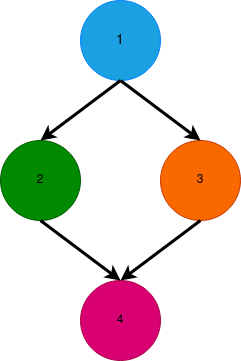
\includegraphics[scale=0.7]{Figures/reuse_example_graph.png}
\decoRule
\caption[reuseGraph]{Example of a graph with data reuse}
\label{fig:reuseGraph}
\end{figure}

OnSRAM-Static, the static DNN graph based SPM manager is described as follows.
A graph of operations that represents a DNN is passed to OnSRAM-Static as an
input. All input and output data tensors of each node is analyzed for the start
time, end time, number of reuses, distance between reuses, and size of the
tensor. A weighted sum of these properties is calculated for each tensor to
determine a metric for the cost incurred should a tensor be saved back to main
memory and reloaded onto the SPM again. Based on the graph execution schedule,
the tensors are psuedo-sorted in cost order. They are psuedo-sorted since
tensors that do not overlap in their lifetimes do not need to be sorted relative to
each other. These sorted tensors are then considered in a greedy fashion where
tensors of the highest cost are considered for pinning first. Tensors are only
pinned if they can be pinned for the entire duration of their lifetime without
obstructing tensors needed for other operations before their next reuse. Figure
\ref{fig:onsram_stack} shows an overview of how OnSRAM fits as a compiler extension
into deep learning frameworks.

\begin{figure}[thb]
\centering
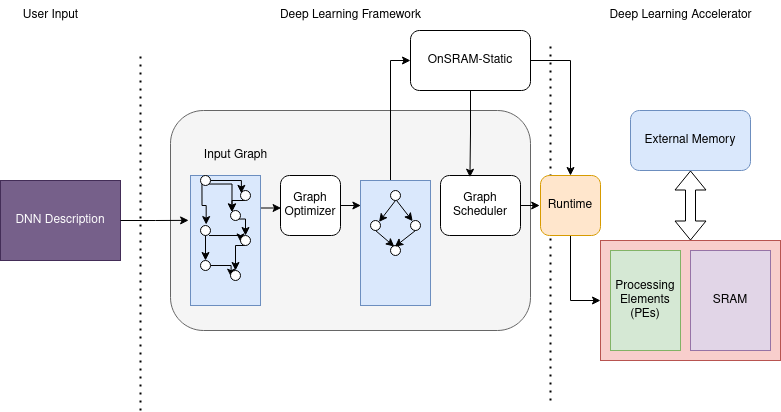
\includegraphics[scale=0.5]{Figures/onsram_stack.png}
\decoRule
\caption[onsramStack]{Overview of OnSRAM}
\label{fig:onsram_stack}
\end{figure}


OnSRAM-Static only applies to input and output tensors, not weights. This is
due to the fact that weights are single use objects that are only needed for
the layers they are used in. There exists no reuse opportunity unlike output
tensors since all layers contain independently different weights. Thus, weights
are not considered for pinning for both OnSRAM-Static and our extension work as
well.

Another aspect that OnSRAM does not consider is applicability towards training.
The assumptions of the problem change when considering training and
significantly increase the difficulty and search space for an optimal solution.
This requires separate compiler extension implementations to be designed into
separate portions of the framework. Further, batched training, partitioned
accelerators, distributed systems, and large reuse distances due to backward
passes and batched data \cite{onsram} bring significant design challenges that
are not present in inference. Thus we have also chosen not to extend this work
in this regard as well.

%----------------------------------------------------------------------------------------
%	SECTION 2
%----------------------------------------------------------------------------------------

\section{Simulation and Architecture}
% how important is this question? should we just be saying what we used

Differences in hardware and simulators don't affect the relative performance of
a non-pinning compiler compared to a pinning compiler if the model, inputs,
framework, and hardware stay constant. However there are some important
environment variables that will consequently affect repeatability and benchmark
performance. Most notably, the simulator and hardware architecture in use.

OnSRAM uses a cycle accurate simulator to model and assess the performance of
their algorithm \cite{onsram}.  We have opted to use the SMAUG\cite{smaug}
framework that depends on the gem5 Aladdin\cite{aladdin} system to model our
accelerator and implement our experiments.
While gem5 is not cycle accurate, it still advertises a close to cycle accurate
performance metrics and creates a relative base of comparison between base
models and our optimized model.

% TODO: explain smaug more. like what it is and stuff and like other stuff from
% the paper

Intra-node optimizations that both simulators do but may not do the same way
that may affect performance comparisons: loop tiling, loop ordering, unrolling,
node re-ordering, and pipelined DMA operations for maximizing intra-node reuse.

% architectural differences
We use the default SMAUG provided accelerator inspired by NVDLA\cite{smaug}.
The accelerator contains eight PEs, multiply accumalate (MACC) arrays, and
contains 3 scratchpad memories\cite{smaug}. Two scratchpads are configured to
be used as inputs and one for output. Each scratchpad is sized at 32Kb as a default
configuration.

%----------------------------------------------------------------------------------------
%	SECTION 3
%----------------------------------------------------------------------------------------

\section{Extensions}

%-----------------------------------
%	SUBSECTION 1
%-----------------------------------

\subsection{OnSRAM Limitations}

While OnSRAM has contributed a novel SPM management scheme that no framework
has explored to date \cite{onsram}, there are limitations that do not allow it to
generalize in a hardware agnostic scenario. This is due to its assumption that
the accelerator contains only one shared scratchpad for input and output
tensors. A consequence of this is that the greedy algorithm proposed to map
possible pin candidates is non-trivial to apply to an accelerator with more
than one scratchpad. Further, because of the heuristic approach, OnSRAM is not
able to achieve the optimal memory mappings with respect to minimizing memory
transfer.

%-----------------------------------
%	SUBSECTION 2
%-----------------------------------

\subsection{Motivating Example}

% explain how onsram does the thing

Consider the computational graph of in figure 1. The graph clearly shows that
node 0's output will be reused as inputs to node 1 and 2. In a single SPM case,
we can see how the tensors would be mapped for each timestep. Clearly, the
leftover space of the SPM is what we can use as leftover pinning space between
operations. However, in the case of a multi-SPM architecture, this is not the
case as tensors cannot be split over different SPMs. To effectively navigate
the optimal mapping of pinned tensors, what SPM a tensor is pinned on greatly
affects the accumulated number of data transfers because of its effect on the
mapping of future tensors to an SPM. Once a tensor is pinned to a particular
SPM, mappings of inputs and outputs associated to other operations must be
remapped in accordance to the remaining capacity of all SPMs. This issue can be
compared to the bin-packing problem where the SPMs are bins and the tensors are
the items. Hence, for every possible mapping of a particular tensor to a SPM,
there exists new mapping for all other tensors that will exist for that
particular operation and future operations relative to the position of the
pinned tensor. The combinatorial explosion of possible mappings of tensors,
how long each one is mapped for, and where they are mapped is a search space
that grows with the depth of the deep learning model. A model of such
a mapping problem is shown in figure 3.

Notably, the single SPM case does not involve the concern of the exact location for
pinning a tensor. Rather, the decision making process in such a case is guided
solely by a tesnor's relative cost, its size, and the degree of overlap it has
with other tensors in terms of liveness. These factors shape how a pinned
tensor could influence future pinning opportunities for other tensors.
Due to these new considerations, simply porting the OnSRAM greedy algorithm 
leads to inefficient results since only a single scratchpad in the DLA can
be used for pinning.

Rather than porting the OnSRAM approach; utilizing a naively greedy approach in
the context of multiple SPMs, i.e., initially pinning an item to whatever SPM
has the most space and remapping the inputs and outputs accordingly, has also
been considered. This process involves pinning outputs of every operation and
evicting the tensors when the pinned tensor cannot accommodate all other
necessary tensors for an operation, or when the output of the present operation
is of higher importance. The initial decision of selecting an SPM to pin an
item, which depends on the primary remapping of inputs and outputs around a
pinned tensor, can considerably influence the pinnability of future items. This
might, in certain instances, lead to the unpinned state of items immediately
prior to their reuse.

In such an approach, the system may not adequately identify opportunities for
reuse, leading to unpredictable decision-making and near-suboptimal results.
This limitation persists, albeit in a reduced form, even when the size of the
SPMs are increased. Therefore, to devise an algorithm that meticulously analyzes
possible decisions and maps tensors in a manner that effectively encourages
reuse, one could implement techniques such as graph coloring or ILP, which are
similar to the methods used in solving the pseudo-register SPM register
allocation problem.

Choosing an optimal pinning strategy to minimize the amount of data transfers
within this search space is the goal of this work.


\begin{figure}[th]
\centering
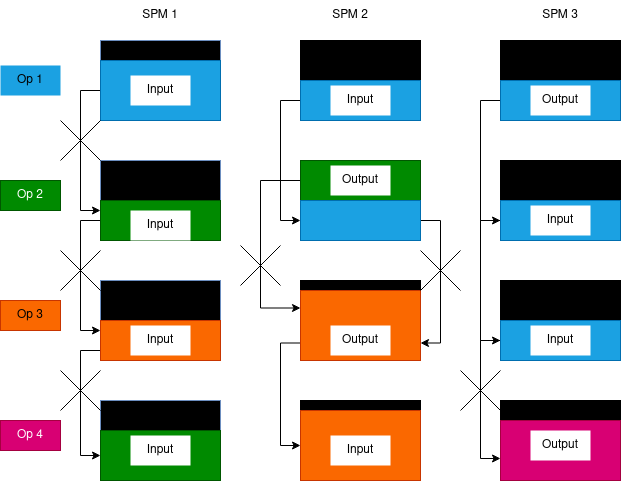
\includegraphics[scale=0.7]{Figures/reuse_example_pin_map_fail_1.png}
\decoRule
\caption[pin_naive]{Example of a un-optimal pinning strategy}
\label{fig:pin_naive}
\end{figure}


\begin{figure}[th]
\centering
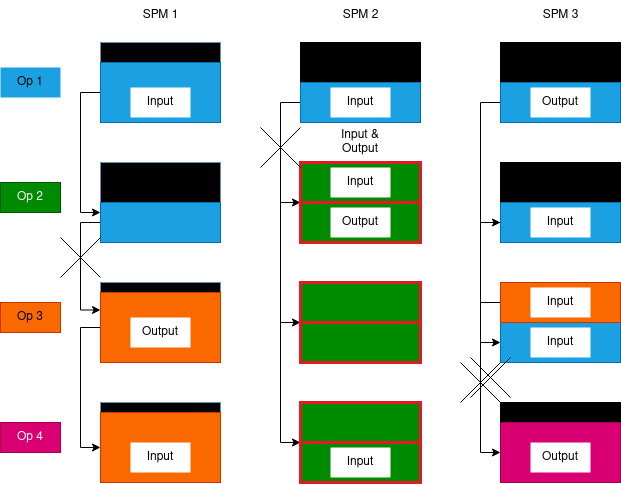
\includegraphics[scale=0.7]{Figures/reuse_example_pin_all.png}
\decoRule
\caption[pin_optimal]{Example of an optimal pinning strategy}
\label{fig:pin_optimal}
\end{figure}

\subsection{Proposed Approach}
% we do everything in the 3 spm case
% goal is to mitigate data transfers between SPMs and main memory
% In order to analyze the possible mapping
In order to analyze the search space and create a pin mapping for all tensors
such that the number of data transfers between SPMs and main memory on an
inter-node graph level are minimized, we propose an ILP model to create an
optimal strategy for a multi-scratchpad architecture.

To do this we first take an optimized computational graph and create a final
schedule of operators that will be ran. Using this schedule of operators, we
then aggregate all tensors that are used in the DNN. Each input and output
tensor is annotated with the operator from which it was created and all
operators that require it as a dependency. All tensor sizes, number of SPMs,
and the size of the SPMs are gathered as well. Using this information an
initial naive mapping scheme can be created where all inputs and outputs are
mapped to a designated input SPM and output SPM. All outputs are assumed to be
saved back to memory and reloaded when needed. We then use the initial mapping
as an input into the ILP solver to realize the optimal strategy.
